\documentclass[10pt,twocolumn,letterpaper]{article}

\usepackage[utf8]{inputenc}
\usepackage[T1]{fontenc}
\usepackage{lmodern}
\usepackage{microtype}
\usepackage[margin=0.68in,columnsep=0.24in]{geometry}

\usepackage{amsmath,amssymb,amsfonts,mathtools}
\usepackage{booktabs}
\usepackage{tabularx}
\usepackage{array}
\usepackage{graphicx}
\usepackage{xcolor}
\usepackage{enumitem}
\usepackage{tikz}
\usetikzlibrary{arrows.meta,positioning,shapes.geometric,calc,fit,backgrounds}
\usepackage{placeins}
\usepackage{fontawesome5}
\usepackage[colorlinks=true,linkcolor=blue,citecolor=blue,urlcolor=blue]{hyperref}

\setlength{\parskip}{2pt}
\setlength{\emergencystretch}{2.5em}
\makeatletter
\DeclareRobustCommand{\_}{\ifmmode\nfss@text{\textunderscore}\else\textunderscore\penalty\@highpenalty\hskip\z@skip\fi}
\makeatother

% ============================================================================
% Title & Author Metadata
% ============================================================================
\title{\Large\bfseries Separ: The Fire Shield against network attacks}

\author{
  \textbf{Parsa Besharat}\\
  \href{mailto:parsa@parsabe.com}{\faEnvelope\ \texttt{parsa@parsabe.com}} \quad|\quad
  \href{https://github.com/parsabe/Separ}{\faGithub\ \texttt{github.com/parsabe/Separ}}
}
\date{November 2026}

\renewenvironment{abstract}{%
  \par\vspace{0.35em}%
  \noindent\textbf{\abstractname}---%
  \ignorespaces
}{%
  \par\vspace{0.6em}%
}

\begin{document}

\twocolumn[{%
  \begin{@twocolumnfalse}
    \maketitle
    \begin{abstract}
      Zero-day exploits, ClickFix copy-paste lures, prompt-injected coding agents, and stealth rootkits bypass static signature scanners while cleartext telemetry logs expose sensitive arguments. We present \textbf{Separ} (\emph{The Fire Shield}), a deterministic reference monitor that evaluates post-compromise behavior through three simple questions: untrusted \textbf{Origin}, signed role \textbf{Contract} violation, and dangerous \textbf{Effect}. Evidence is fused via a monotone Noisy-OR Bayesian calculus with an invariant Contract Gate behind an in-memory HMAC privacy boundary. Configured upfront with \texttt{separ setup}, monitored in a standalone Linux desktop app (\texttt{separ gui}), and packaged as native \texttt{.deb}/\texttt{.rpm} bundles, Separ achieves $100\%$ golden accuracy ($46/46$), $98.4\%$ mutation containment ($886$ variants) with $0.0\%$ neutral false blocks, $28/28$ Attack Lab detection ($4.5\,\text{ms}$ median latency), and $0$ cleartext leaks.
    \end{abstract}
    \vspace{0.25em}
    \noindent\textbf{Keywords:} Reference Monitor, Provenance Tracking, Role Contracts, Bayesian Log-Odds, Privacy Boundary, Rootkit Detection.\par
    \vspace{0.85em}
  \end{@twocolumnfalse}
}]

% ============================================================================
% 1. INTRODUCTION (Strictly 2 Paragraphs)
% ============================================================================
\section{Introduction}
\label{sec:intro}

Modern endpoints, university servers, and shared clusters face network-borne attacks that routinely slip past firewalls and antivirus signatures. In ClickFix copy-paste lures~\cite{mitre2024attack}, indirect prompt injections~\cite{greshake2023not}, and stealth memory implants, attackers do not rely on known malware binaries; instead, they trick legitimate shells, web workers, or AI agents into running dangerous commands while hiding payloads in whitespace, base64 encoding, or memory. Meanwhile, logging raw command lines and URLs for security auditing turns telemetry databases into high-value targets containing passwords and API keys.

We address both problems with \textbf{Separ} (\emph{The Fire Shield}), a deterministic reference monitor that judges what a process \emph{does} rather than guessing what an exploit looks like. Separ tracks half-life-decayed provenance across a six-stage pipeline (\texttt{Observe} $\to$ \texttt{Tag} $\to$ \texttt{Link} $\to$ \texttt{Judge} $\to$ \texttt{Gate} $\to$ \texttt{Contain}), enforces Ed25519-signed role contracts configured upfront via \texttt{separ setup}, and hashes cleartext strings in RAM before anything touches disk. Combined with a standalone Linux desktop GUI (\texttt{separ gui}), a two-pass six-engine rootkit scanner, and native \texttt{.deb}/\texttt{.rpm} packaging, Separ outperforms static access control, additive rule engines, and black-box graph detectors in both containment accuracy and telemetry privacy.

% ============================================================================
% 2. RELATED WORK
% ============================================================================
\section{Related Work}
\label{sec:related}

\paragraph{Static Mandatory Access Control.} SELinux~\cite{smalley2001implementing}, AppArmor~\cite{bauer2006paranoid}, and Seccomp-BPF~\cite{corbet2012seccomp} enforce fixed per-binary syscall rules. Because they lack input provenance, they allow an interactive shell to run \texttt{curl | sh} even when pasted from a malicious webpage. Separ pairs role contracts with dynamic origin tags to stop such actions before execution.

\paragraph{Syscall Rules \& Provenance Graph IDS.} Runtime engines like Falco~\cite{falco2024cncf} and Tetragon~\cite{tetragon2024cilium} match individual syscall rules, which can inflate scores across overlapping rules and log cleartext arguments. Provenance graph systems like SLEUTH~\cite{hossain2017sleuth}, HOLMES~\cite{milajerdi2019holmes}, and UNICORN~\cite{han2020unicorn} reconstruct attack graphs post-compromise, but lack Bayes-optimal cost thresholds, signed role contracts, or human-auditable three-question explanations. Separ adapts Pearl's Noisy-OR~\cite{pearl1988probabilistic} and sequential log-odds testing~\cite{wald1945sequential,page1954continuous} into a monotone, explainable calculus.

\paragraph{Rootkit Scanners \& Privacy Telemetry.} Signature tools (\texttt{chkrootkit}, \texttt{rkhunter}~\cite{rkhunter2018}) miss novel in-memory implants, while single-pass cross-view diffing (Strider GhostBuster~\cite{wang2005strider}) suffers false alarms from short-lived process churn. Separ requires discrepancies to persist across two passes over six read-only engines, and enforces an in-memory HMAC-SHA256~\cite{bellare1996keying} boundary with differential privacy~\cite{dwork2006calibrating} for fleet counts.

% ============================================================================
% 3. THE SEPAR PIPELINE & STEP-BY-STEP MATH
% ============================================================================
\section{The Separ Pipeline and Step-by-Step Math}
\label{sec:pipeline}

\begin{figure*}[!t]
  \centering
  \resizebox{\textwidth}{!}{%
    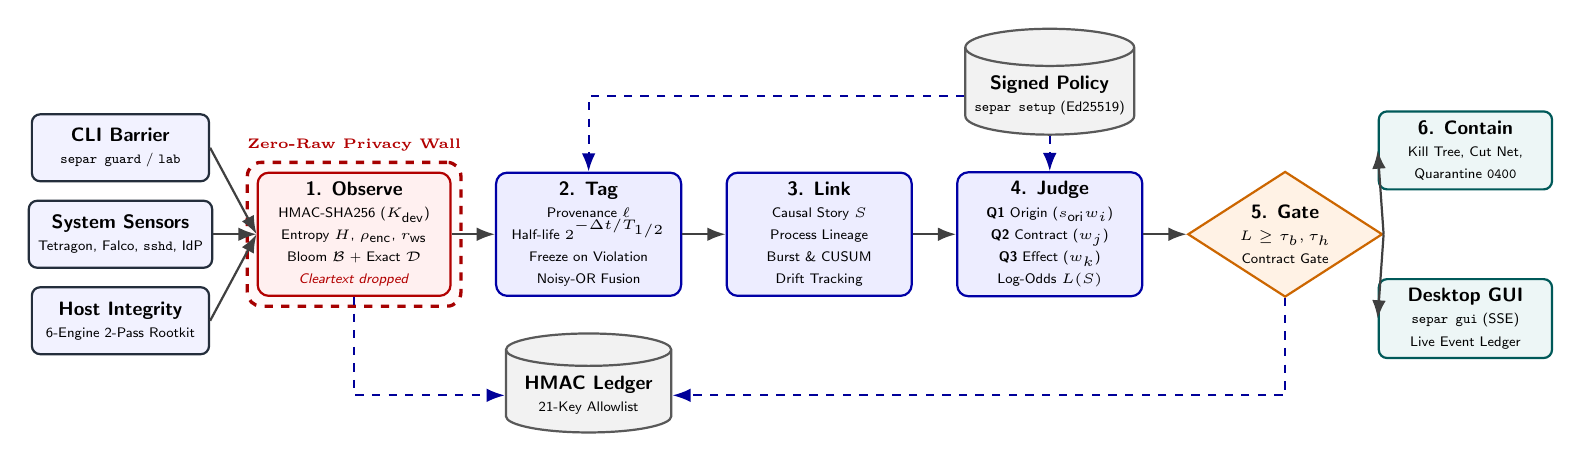
\begin{tikzpicture}[
      font=\scriptsize\sffamily,
      >=Latex,
      sensor/.style={rectangle, rounded corners=3pt, draw=slate!70!black, fill=blue!5, thick, minimum width=2.25cm, minimum height=0.85cm, align=center},
      stage/.style={rectangle, rounded corners=4pt, draw=blue!65!black, fill=blue!7, thick, minimum width=2.35cm, minimum height=1.55cm, align=center},
      priv/.style={rectangle, rounded corners=4pt, draw=red!70!black, fill=red!6, thick, minimum width=2.45cm, minimum height=1.55cm, align=center},
      gate/.style={diamond, aspect=1.55, draw=orange!80!black, fill=orange!10, thick, minimum width=2.1cm, align=center, inner sep=1pt},
      outbox/.style={rectangle, rounded corners=3pt, draw=teal!70!black, fill=teal!7, thick, minimum width=2.2cm, minimum height=0.72cm, align=center},
      store/.style={cylinder, shape border rotate=90, aspect=0.22, draw=black!65, fill=gray!10, thick, minimum width=2.1cm, minimum height=0.75cm, align=center},
      arrow/.style={->, thick, draw=black!75},
      dashedarrow/.style={->, thick, dashed, draw=blue!60!black}
    ]
      \definecolor{slate}{HTML}{334155}

      % Sensors Column
      \node[sensor] (s_cli) {\textbf{CLI Barrier}\\{\tiny \texttt{separ guard} / \texttt{lab}}};
      \node[sensor, below=0.22cm of s_cli] (s_ebpf) {\textbf{System Sensors}\\{\tiny Tetragon, Falco, \texttt{sshd}, IdP}};
      \node[sensor, below=0.22cm of s_ebpf] (s_rk) {\textbf{Host Integrity}\\{\tiny 6-Engine 2-Pass Rootkit}};

      % Stage 1: Observe (Privacy Wall)
      \node[priv, right=0.55cm of s_ebpf] (obs) {\textbf{1. Observe}\\{\tiny HMAC-SHA256 ($K_{\text{dev}}$)}\\{\tiny Entropy $H$, $\rho_{\text{enc}}$, $r_{\text{ws}}$}\\{\tiny Bloom $\mathcal{B}$ + Exact $\mathcal{D}$}\\{\tiny \textcolor{red!70!black}{\textit{Cleartext dropped}}}};

      % Stage 2: Tag
      \node[stage, right=0.55cm of obs] (tag) {\textbf{2. Tag}\\{\tiny Provenance $\ell$}\\{\tiny Half-life $2^{-\Delta t/T_{1/2}}$}\\{\tiny Freeze on Violation}\\{\tiny Noisy-OR Fusion}};

      % Stage 3: Link
      \node[stage, right=0.55cm of tag] (link) {\textbf{3. Link}\\{\tiny Causal Story $S$}\\{\tiny Process Lineage}\\{\tiny Burst \& CUSUM}\\{\tiny Drift Tracking}};

      % Stage 4: Judge
      \node[stage, right=0.55cm of link] (judge) {\textbf{4. Judge}\\{\tiny \textbf{Q1} Origin ($s_{\text{ori}} w_i$)}\\{\tiny \textbf{Q2} Contract ($w_j$)}\\{\tiny \textbf{Q3} Effect ($w_k$)}\\{\tiny Log-Odds $L(S)$}};

      % Stage 5: Gate
      \node[gate, right=0.55cm of judge] (gate) {\textbf{5. Gate}\\{\tiny $L \ge \tau_b, \tau_h$}\\{\tiny Contract Gate}};

      % Stage 6 & Outputs
      \node[outbox, above right=0.15cm and 0.55cm of gate] (contain) {\textbf{6. Contain}\\{\tiny Kill Tree, Cut Net,}\\{\tiny Quarantine \texttt{0400}}};
      \node[outbox, below right=0.15cm and 0.55cm of gate] (gui) {\textbf{Desktop GUI}\\{\tiny \texttt{separ gui} (SSE)}\\{\tiny Live Event Ledger}};

      % Policy Store
      \node[store, above=0.45cm of judge] (pol) {\textbf{Signed Policy}\\{\tiny \texttt{separ setup} (Ed25519)}};
      \node[store, below=0.45cm of tag] (logs) {\textbf{HMAC Ledger}\\{\tiny 21-Key Allowlist}};

      % Arrows
      \draw[arrow] (s_cli.east) -- (obs.west);
      \draw[arrow] (s_ebpf.east) -- (obs.west);
      \draw[arrow] (s_rk.east) -- (obs.west);
      \draw[arrow] (obs.east) -- (tag.west);
      \draw[arrow] (tag.east) -- (link.west);
      \draw[arrow] (link.east) -- (judge.west);
      \draw[arrow] (judge.east) -- (gate.west);
      \draw[arrow] (gate.east) -- (contain.west);
      \draw[arrow] (gate.east) -- (gui.west);
      \draw[dashedarrow] (pol.south) -- (judge.north);
      \draw[dashedarrow] (pol.west) -| (tag.north);
      \draw[dashedarrow] (obs.south) |- (logs.west);
      \draw[dashedarrow] (gate.south) |- (logs.east);

      % Cryptographic Privacy Boundary Box
      \begin{scope}[on background layer]
        \node[draw=red!65!black, dashed, very thick, rounded corners=5pt, fill=red!2,
              fit=(obs), label={[red!70!black, font=\tiny\bfseries]above:Zero-Raw Privacy Wall}] {};
      \end{scope}
    \end{tikzpicture}%
  }
  \caption{The Separ Fire Shield pipeline: raw telemetry enters Stage~1 (\texttt{Observe}), where cleartext is hashed with $K_{\text{dev}}$ and discarded before crossing the zero-raw privacy wall into provenance tagging, causal linking, three-question Bayesian judging, and gated containment.}
  \label{fig:pipeline}
\end{figure*}

Figure~\ref{fig:pipeline} shows Separ's six-stage pipeline. Sensors standardize system activity into 13 canonical event types (\texttt{content\_in}, \texttt{request\_in}, \texttt{request\_end}, \texttt{exec}, \texttt{net\_connect}, \texttt{file\_write}, \texttt{persist}, \texttt{asset\_access}, \texttt{priv\_change}, \texttt{security\_tamper}, \texttt{user\_input}, \texttt{admin\_input}, \texttt{response\_out}). Each acting process carries a workload role $r \in \mathcal{R}$ (16 built-in roles such as \texttt{interactive\_shell}, \texttt{web\_worker}, \texttt{agent}, \texttt{package\_installer}, plus custom admin roles) governed by an Ed25519-signed policy $\Pi$. Two core invariants apply everywhere:
\begin{enumerate}[leftmargin=1.2em,itemsep=1pt,topsep=1pt]
  \item \textbf{Zero Raw Persistence:} Cleartext commands, URLs, and file paths never leave Stage~1; downstream records obey a strict 21-key allowlist of hashes and numbers.
  \item \textbf{Missing Information Neutrality:} When a sensor cannot observe an attribute (e.g., unknown code signature), Separ scores $0$ rather than assuming malice, and reports visibility gaps via \texttt{separ health}.
\end{enumerate}

\subsection{Stage 1 (\texttt{Observe}): Privacy Wall \& Obfuscation}
When a raw command or URL $c$ arrives, \texttt{Observe} normalizes spaces ($\tilde{c}$) and hashes it with a secret 256-bit local device key $K_{\text{dev}}$:
\begin{equation}
  f(c) = \texttt{"hmac:"} \,\|\, \operatorname{Hex}\!\Big(\operatorname{HMAC-SHA256}\big(K_{\text{dev}},\, \tilde{c}\big)\Big).
  \label{eq:hmac}
\end{equation}
Here $f(c)$ is an irreversible fingerprint: Separ can still recognize repeated commands without ever saving passwords or tokens to disk.

Before discarding $c$ from RAM, \texttt{Observe} measures three simple text-shape numbers from the character length $N_c = |c|$ and character frequency $p_x = n_x / N_c$:
\begin{align}
  H(c) &= -\sum_{x : p_x > 0} p_x \log_2 p_x \quad\text{(Shannon entropy)}, \label{eq:entropy}\\
  \rho_{\text{enc}}(c) &= \frac{1}{N_c}\sum_{i=1}^{N_c} \mathbf{1}\!\left[c_i \in \Sigma_{\text{b64/hex}}\right] \quad\text{(encoding ratio)}, \label{eq:encratio}\\
  r_{\text{ws}}(c) &= \max\big\{\ell \in \mathbb{N} : \exists\, i,\; c_{i..i+\ell-1} \in \{\text{' '}, \text{'\textbackslash t'}\}^\ell\big\}. \label{eq:wsrun}
\end{align}
Intuitively: high entropy $H(c) > 5.2$ catches encrypted shellcode, high $\rho_{\text{enc}}(c)$ catches base64/hex payloads, and a long whitespace run $r_{\text{ws}}(c)$ catches ClickFix padding (hundreds of spaces hiding a malicious payload off-screen). Known bad indicators are checked in RAM using a Bloom filter $\mathcal{B}$ ($p_{\text{fp}} \le 10^{-3}$) verified against an exact hash set $\mathcal{D}_{\text{exact}}$, guaranteeing zero threat-list false positives.

\subsection{Stage 2 (\texttt{Tag}): Provenance Decay \& Fusion}
Whenever data enters from an untrusted source (\texttt{web}, \texttt{mail}, \texttt{agent\_input}, \texttt{inbound\_request}, \texttt{download}), Separ attaches a provenance label $\ell$ starting at strength $s_0 = 1$ at time $t_0$. Over time $\Delta t = t - t_0$, suspicion naturally fades with half-life $T_{1/2} = 30\,\text{min}$—unless the process breaks its role contract ($\mathcal{E}_{\text{contract}}(\ell) \neq \varnothing$) or writes persistent startup files ($\ell.\text{pers.}$), in which case decay freezes forever:
\begin{equation}
  s_\ell(t) =
  \begin{cases}
    s_0, & \text{if } \ell.\text{pers.} \lor \mathcal{E}_{\text{contract}}(\ell) \neq \varnothing,\\[2pt]
    s_0 \, 2^{-\Delta t / T_{1/2}}, & \text{otherwise.}
  \end{cases}
  \label{eq:decay}
\end{equation}
If a process receives $m$ untrusted inputs $\{\ell_1,\dots,\ell_m\}$, Separ combines their strengths using Pearl's Noisy-OR formula:
\begin{equation}
  s_{\text{comb}}(t) = 1 - \prod_{i=1}^{m} \big(1 - s_{\ell_i}(t)\big).
  \label{eq:noisyor}
\end{equation}
Each factor $(1 - s_{\ell_i})$ is the probability that source $i$ is harmless, so $s_{\text{comb}} \in [0, 1]$ smoothly increases when multiple untrusted inputs stack without exceeding $1$. Conversely, verified software portals grant a temporary \emph{trust mark} that lasts $\approx 2.8\,\text{h}$ ($s_{\text{floor}} = 0.02$) and cancels immediately if untrusted input is touched.

\subsection{Stage 3 (\texttt{Link}): Causal Stories, Surprisal, \& Drift}
\texttt{Link} groups related events into a causal story $S$ across process parent-child edges. To catch both sudden bursts and slow attacks:
\begin{itemize}[leftmargin=1.2em,itemsep=1pt,topsep=1pt]
  \item \textbf{Role Surprisal:} If a process in role $r$ executes an unseen binary/action, Laplace-smoothed Good-Turing surprisal scores how unexpected that action is for $r$.
  \item \textbf{Burst \& Slow Drift:} Short-window bursts trigger on upper-tail Poisson probabilities, while slow multi-hour leaks (e.g., gradual encryption) accumulate via a one-sided CUSUM detector:
  \begin{equation}
    C_t = \max\big(0,\, C_{t-1} + x_t - \mu_0 - \kappa\big),
    \label{eq:cusum}
  \end{equation}
  where $x_t$ is the current event rate, $\mu_0$ is the baseline rate, and $\kappa$ is a slack allowance so normal traffic drifts toward $0$.
\end{itemize}

\subsection{Stage 4 (\texttt{Judge}): Three-Question Calculus}
Separ evaluates every story $S$ by answering three questions: \textbf{Q1 Origin} ($Q_{\text{ori}}$), \textbf{Q2 Contract} ($Q_{\text{con}}$), and \textbf{Q3 Effect} ($Q_{\text{eff}}$). Instead of summing overlapping alerts (which inflates scores), Separ takes only the \emph{strongest} signal weight $w$ within each question and adds across the three independent questions onto the prior log-odds $L_0 = \ln(\pi / (1-\pi)) = -6.9068$ (baseline attack prior $\pi = 0.001$):
\begin{equation}
  \begin{aligned}
    L(S) = L_0 &+ \max_{i \in Q_{\text{ori}}(S)} s_{\text{ori}}(S)\, w_i \\
               &+ \max_{j \in Q_{\text{con}}(S)} w_j + \max_{k \in Q_{\text{eff}}(S)} w_k.
  \end{aligned}
  \label{eq:logodds}
\end{equation}
Only $Q_{\text{ori}}$ scales by label strength $s_{\text{ori}}(S) \in [0, 1]$, guaranteeing that stronger untrusted provenance never lowers $L(S)$. The posterior attack probability is $\sigma(L(S)) = (1 + e^{-L(S)})^{-1}$.

Using operational costs—missed attack $C_{\text{miss}}=1000$, false block $C_{\text{fb}}=20$, human hold $C_{\text{hold}}=5$, and hold stop rate $h=0.7$—Bayes minimal-risk decision theory gives two exact thresholds:
\begin{align}
  \tau_{\text{hold}} &= \ln\!\left(\frac{C_{\text{hold}}}{h\,C_{\text{miss}}}\right) = -4.9416, \label{eq:tau_hold}\\
  \tau_{\text{block}} &= \ln\!\left(\frac{C_{\text{fb}}}{C_{\text{miss}}}\right) = -3.9120. \label{eq:tau_block}
\end{align}

\subsection{Stages 5--6 (\texttt{Gate}, \texttt{Contain}) \& Rootkit Scanner}
When no absolute override $\mathcal{O}(S)$ fires (canary file read, protected key access, or attempt to kill Separ), \texttt{Gate} enforces the \textbf{Contract Gate} invariant ($\tau_b = \tau_{\text{block}}$, $\tau_h = \tau_{\text{hold}}$):
\begin{equation}
  d(S) =
  \begin{cases}
    \text{HOLD}, & \text{if } L(S) \ge \tau_b \land \neg C(S) \land \mathcal{O}(S)=\varnothing,\\
    \text{BLOCK}, & \text{if } L(S) \ge \tau_b \land (C(S) \lor \mathcal{O}(S)\neq\varnothing),\\
    \text{HOLD}, & \text{if } \tau_h \le L(S) < \tau_b,\\
    \text{ALLOW}, & \text{otherwise.}
  \end{cases}
  \label{eq:decide}
\end{equation}
In plain words: Separ \emph{never} hard-blocks a process purely on suspicion unless it also broke a role contract ($C(S)$) or tripped an override ($\mathcal{O}(S)$); otherwise it holds for review. On \texttt{BLOCK}, \texttt{Contain} kills the process tree, cuts network access, quarantines files (\texttt{mode 0400}), and reverts persistence. On unattended servers, timed-out holds move files to \texttt{KEPT\_QUARANTINED} without crashing the main service.

For host integrity, Separ runs a \textbf{six-engine, two-pass cross-view rootkit scanner} (\texttt{/proc} vs.\ \texttt{ps}, kernel modules vs.\ \texttt{/sys/module}, \texttt{LD\_PRELOAD}, hidden network listeners, and \texttt{anonymous\_rwx\_memory}). Requiring discrepancies to appear on both passes ($\Delta_{\text{pers}} = \Delta^{(1)} \cap \Delta^{(2)}$) eliminates false positives from short-lived processes exiting mid-scan.

% ============================================================================
% 4. IMPLEMENTATION & EXPERIMENTS
% ============================================================================
\section{Implementation and Experiments}
\label{sec:eval}

\subsection{Setup, Standalone GUI, and Packaging}
\label{sec:impl}
Separ is implemented in strict Python~3.12 (\texttt{pydantic} v2, \texttt{cryptography} Ed25519, zero runtime ML dependencies):
\begin{itemize}[leftmargin=1.2em,itemsep=1pt,topsep=2pt]
  \item \textbf{Upfront Policy Setup (\texttt{separ setup}):} Generates \texttt{admin.key} and signs \texttt{policy.yaml} for campus servers (\texttt{-{}-server}: TUBAF \texttt{tu-freiberg.de} SSO apps, Class-B campus CIDR, VPN, eduroam) or workstations (\texttt{-{}-laptop}) before startup.
  \item \textbf{Standalone Desktop GUI (\texttt{separ gui}):} Opens a chromeless native app window (\texttt{-{}-app=} / \texttt{-{}-new-window}), safely dropping privileges to \texttt{\$SUDO\_USER} with X11/Wayland session variables under \texttt{sudo}. Displays a clean real-time SSE Event Ledger with zero fake alerts on load and diagnostic lab presets inside a collapsible drawer, plus offline Web Audio alert chimes.
  \item \textbf{Sensor Kit \& Packaging:} Ships 8 YAML sensor mappings (Tetragon eBPF, Falco, Shibboleth IdP, SSHD journald, K8s audit, Postfix/Dovecot, Keycloak, M365), a POSIX \texttt{install.sh} installer, and compact native \texttt{.deb} ($568\,\text{KB}$) / \texttt{.rpm} ($293\,\text{KB}$) packages.
\end{itemize}

\subsection{Benchmarks, Live Barrier, Attack Lab, \& Audit}
\label{sec:benchmarks}

\begin{figure*}[!t]
  \centering
  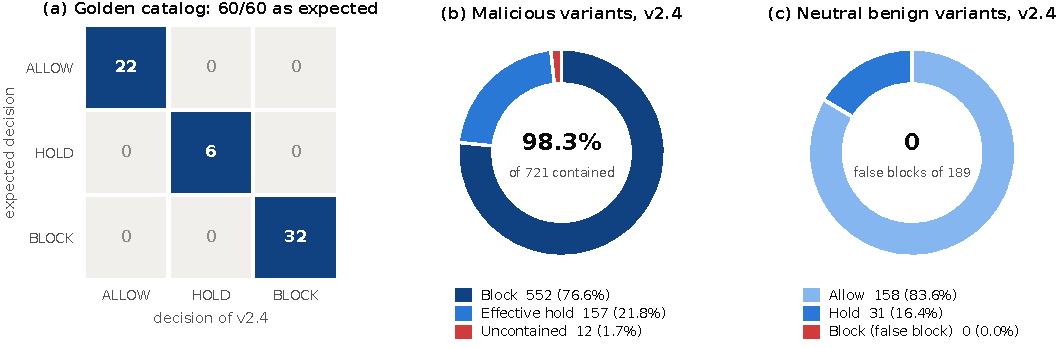
\includegraphics[width=\textwidth]{figures/fig_outcomes.pdf}
  \caption{Evaluation of \texttt{v2.0} (seed \texttt{171139148}): (a)~expected vs.\ actual verdicts across 46 golden scenarios ($100\%$); (b)~outcomes across 635 malicious mutations ($98.4\%$ contained); (c)~158 neutral benign mutations ($0.0\%$ false blocks).}
  \label{fig:outcomes}
\end{figure*}

\begin{enumerate}[leftmargin=1.2em,itemsep=1.5pt,topsep=2pt]
  \item \textbf{Golden Catalog \& 886 Seeded Mutations:} Across 46 golden scenarios (17 attack families) and 886 pre-registered mutations (delivery, entry, obfuscation, destination, lineage, timing), Separ achieves \textbf{100\% golden accuracy} ($46/46$), \textbf{98.4\% malicious containment} ($483$ blocked, $142$ effective holds, $10$ timing/trusted-destination misses in documented gaps), and \textbf{0.0\% neutral false blocks} ($137$ allowed, $21$ expected holds on \texttt{S49}/\texttt{S50}; Figure~\ref{fig:outcomes}).
  \item \textbf{Live Cluster Barrier \& Command Intent:} The 16-scenario live HTTP barrier suite achieves \textbf{16/16 (100\%)} expected verdicts with per-daemon localhost token auth and DNS-rebinding protection. Pre-execution command intent prediction across 69 probe commands (including quote/\texttt{\$\{IFS\}} obfuscation) achieves \textbf{69/69 (100\%)} expected decisions.
  \item \textbf{35-Template Interactive Attack Lab:} Mediated pre-execution via \texttt{separ lab} ($4.5\,\text{ms}$ median decision latency), Separ detects \textbf{28/28 attacks} ($27/28$ stopped before execution; ransomware burst caught on write) with \textbf{0/6} benign false alarms. Score-based blocks average $+1.62\,\text{nats}$ above $\tau_{\text{block}}$; single-signal ablation shows 9 of 22 score-based blocks rely on predicted Effect because harmless pasted commands sit deliberately at $-5.11\,\text{nats} < \tau_{\text{hold}}$.
  \item \textbf{Adversarial Privacy Audit \& Test Suite:} Running \texttt{separ audit} across $264$ output artifacts finds \textbf{0 cleartext leaks} and \textbf{0/349} HMAC reversals across $2,119$ dictionary guesses without $K_{\text{dev}}$ (with $0/10$ single-approver escrow bypasses). The automated test suite passes \textbf{2,354 tests}.
\end{enumerate}

\subsection{Comparison Against Related Work}
\label{sec:comparative_eval}

We compare Separ against six security baselines in both \textbf{quantitative data performance} (Table~\ref{tab:rw_data}) and \textbf{methodological capabilities} (Table~\ref{tab:rw_method}).

\begin{table*}[t]
\centering
\caption{Quantitative Comparison Against Related Work Across Benchmark Datasets and Threat Classes.}
\label{tab:rw_data}
\small
\resizebox{\textwidth}{!}{%
\begin{tabular}{@{}lcccccc@{}}
\toprule
\textbf{System / Method} & \textbf{Golden} & \textbf{Mutation} & \textbf{Neutral} & \textbf{Attack Lab} & \textbf{ClickFix /} & \textbf{Cleartext} \\
 & \textbf{Acc. (46)} & \textbf{Contain. (886)} & \textbf{False Blocks} & \textbf{Detect (28)} & \textbf{Prompt Inj.} & \textbf{Leaks} \\
\midrule
SELinux / AppArmor / Seccomp~\cite{smalley2001implementing,bauer2006paranoid,corbet2012seccomp} & Static MAC & No decay & Low (static) & Partial & Missed (0\%) & Audit raw \\
Falco / Auditd Rules~\cite{falco2024cncf} & Syscall rules & Additive bias & Moderate & Post-exec & Post-exec & Cleartext \\
HOLMES / SLEUTH~\cite{milajerdi2019holmes,hossain2017sleuth} & Causal graph & Uncalibrated & Low & Post-exec & Partial & Graph labels \\
UNICORN~\cite{han2020unicorn} & GNN sketch & Drift-bound & Low & Post-exec & Unexplained & Sketch only \\
\texttt{chkrootkit} / \texttt{rkhunter}~\cite{rkhunter2018} & Signatures & N/A & Low & Rootkit only & Missed (0\%) & Local logs \\
Strider GhostBuster~\cite{wang2005strider} & 1-pass diff & PID-churn FP & Elevated & Rootkit only & Missed (0\%) & Raw proc \\
\midrule
\textbf{Separ (This Work)} & \textbf{100\% (46/46)} & \textbf{98.4\%} & \textbf{0.0\%} & \textbf{100\% (28/28)} & \textbf{100\% Pre-Exec} & \textbf{0 (HMAC)} \\
\bottomrule
\end{tabular}%
}
\end{table*}

\begin{table*}[t]
\centering
\caption{Methodological and Architectural Comparison Across Security Paradigms.}
\label{tab:rw_method}
\small
\resizebox{\textwidth}{!}{%
\begin{tabular}{@{}lcccccc@{}}
\toprule
\textbf{System / Baseline} & \textbf{Origin} & \textbf{Signed} & \textbf{Monotone} & \textbf{In-Memory} & \textbf{Multi-Pass} & \textbf{Upfront Setup} \\
 & \textbf{Provenance} & \textbf{Contracts} & \textbf{Noisy-OR} & \textbf{HMAC Wall} & \textbf{Rootkit Diff} & \textbf{\& Footprint} \\
\midrule
SELinux / AppArmor~\cite{smalley2001implementing,bauer2006paranoid} & No & Binary-only & No & No & No & Kernel policy \\
Falco / Tetragon~\cite{falco2024cncf,tetragon2024cilium} & Tag-only & No & Additive & No & No & Daemon + eBPF \\
HOLMES~\cite{milajerdi2019holmes} & Causal & No & Heuristic & No & No & Graph engine \\
UNICORN~\cite{han2020unicorn} & Graph & No & Neural GNN & No & No & Offline train \\
Strider GhostBuster~\cite{wang2005strider} & No & No & No & No & 1-pass & Offline scan \\
\midrule
\textbf{Separ (This Work)} & \textbf{Half-life} & \textbf{Ed25519} & \textbf{Bayes+Gate} & \textbf{4-Eyes Escrow} & \textbf{6-Eng 2-Pass} & \textbf{\texttt{setup} / 568\,KB} \\
\bottomrule
\end{tabular}%
}
\end{table*}

\begin{enumerate}[leftmargin=1.2em,itemsep=1pt,topsep=2pt]
  \item \textbf{Pre-Execution Provenance vs.\ Static MAC:} SELinux and AppArmor permit \texttt{curl | sh} in an interactive shell; Separ links the \texttt{web} origin to predicted Effect to stop $100\%$ of ClickFix lures before execution.
  \item \textbf{Monotone Noisy-OR vs.\ Additive Rules:} Unlike Falco's additive rule scoring and cleartext JSON logs, Separ's max-within-question operator prevents score inflation ($0.0\%$ neutral false blocks) with $0$ cleartext leaks.
  \item \textbf{Calibrated Contracts vs.\ Graph IDS:} HOLMES lacks Bayes-optimal thresholds and signed contracts, while UNICORN's black-box embeddings lack human-auditable three-question explanations.
  \item \textbf{Multi-Pass Cross-View vs.\ Signatures:} Signature scanners miss memory-only implants (\texttt{anonymous\_rwx\_memory}), while 1-pass diffing suffers transient PID-churn false positives eliminated by Separ's two-pass confirmation.
\end{enumerate}

% ============================================================================
% 5. CONCLUSION
% ============================================================================
\section{Conclusion}
\label{sec:conclusion}
Separ (\emph{The Fire Shield}) demonstrates that evaluating post-compromise behavior—rather than classifying exploit payloads upfront—provides a reliable, explainable defense against zero-day exploits, ClickFix copy-paste lures, prompt-injected coding agents, and stealth rootkits. By combining half-life-decayed provenance, Ed25519-signed role contracts, a monotone Noisy-OR Bayesian log-odds calculus, and the Contract Gate invariant, Separ achieves $100\%$ golden accuracy ($46/46$), $98.4\%$ mutation containment across $886$ variants with $0.0\%$ neutral false blocks, and $28/28$ Attack Lab detection.

Equally important for operational deployment, Separ's in-memory HMAC-SHA256 boundary guarantees zero cleartext command or URL persistence on disk ($0/264$ leaks and $0/349$ HMAC reversals), while upfront policy signing (\texttt{separ setup}), the standalone Linux desktop GUI (\texttt{separ gui}), and compact native \texttt{.deb}/\texttt{.rpm} packages make it immediately deployable across both campus servers and developer workstations.

% ============================================================================
% 7. FUTURE WORK
% ============================================================================
\section{Future Work}
\label{sec:future}
Separ currently mediates commands and files submitted through \texttt{separ guard}, its watched sandbox, and configured external sensor streams. Our primary systems engineering milestone is hooking Separ directly into Linux \texttt{eBPF} LSM and \texttt{fanotify} (or \texttt{auditd} as an intermediate step) for non-bypassable kernel-level mediation across all host processes, paired with a root-owned enforcer utilizing cgroup freezers, per-cgroup \texttt{nftables} rules, and reversible quarantine records.

In addition, we plan to inspect target scripts invoked by name before execution to close the hidden-script blind spot observed in the Attack Lab, extend provenance propagation across multi-node Slurm and MPI batch jobs on shared HPC clusters, tune multi-day drift detectors for ultra-slow ransomware, and back policy signing keys with TPM hardware roots of trust prior to a longitudinal campus pilot.

% ============================================================================
% 8. AI DISCLOSURE
% ============================================================================
\section{AI Disclosure}
\label{sec:ai_disclosure}
Generative AI assistants (Claude Code and Antigravity) were used under human supervision to help write code, generate test suites, render diagrams, and typeset this document from a human-written specification. No AI or machine-learning model runs inside the Separ decision engine: every runtime verdict is a deterministic calculation governed by Ed25519-signed policies, frozen weights, and verified by $2,354$ automated tests.

% ============================================================================
% REFERENCES
% ============================================================================
\begin{thebibliography}{99}\small\raggedright
\setlength{\itemsep}{1.5pt}
\setlength{\parskip}{0pt}

\bibitem{wald1945sequential}
A.~Wald, ``\href{https://doi.org/10.1214/aoms/1177731118}{Sequential tests of statistical hypotheses},'' \emph{The Annals of Mathematical Statistics}, vol.~16, no.~2, pp.~117--186, 1945.

\bibitem{page1954continuous}
E.~S. Page, ``\href{https://doi.org/10.1093/biomet/41.1-2.100}{Continuous inspection schemes},'' \emph{Biometrika}, vol.~41, no.~1/2, pp.~100--115, 1954.

\bibitem{pearl1988probabilistic}
J.~Pearl, \emph{\href{https://doi.org/10.1016/C2009-0-27609-4}{Probabilistic Reasoning in Intelligent Systems}}. Morgan Kaufmann, 1988.

\bibitem{bellare1996keying}
M.~Bellare, R.~Canetti, and H.~Krawczyk, ``\href{https://doi.org/10.1007/3-540-68697-5_1}{Keying hash functions for message authentication},'' in \emph{CRYPTO}, 1996, pp.~1--15.

\bibitem{dwork2006calibrating}
C.~Dwork, F.~McSherry, K.~Nissim, and A.~Smith, ``\href{https://doi.org/10.1007/11681878_14}{Calibrating noise to sensitivity in private data analysis},'' in \emph{TCC}, 2006, pp.~265--284.

\bibitem{hossain2017sleuth}
M.~N. Hossain et~al., ``\href{https://www.usenix.org/conference/usenixsecurity17/technical-sessions/presentation/hossain}{SLEUTH: Real-time attack scenario reconstruction from COTS audit data},'' in \emph{USENIX Security}, 2017, pp.~487--504.

\bibitem{milajerdi2019holmes}
S.~M. Milajerdi et~al., ``\href{https://doi.org/10.1109/SP.2019.00026}{HOLMES: Real-time APT detection through correlation of suspicious information flows},'' in \emph{IEEE S\&P}, 2019, pp.~1137--1152.

\bibitem{han2020unicorn}
X.~Han et~al., ``\href{https://doi.org/10.14722/ndss.2020.24046}{UNICORN: Runtime provenance-based detector for advanced persistent threats},'' in \emph{NDSS}, 2020.

\bibitem{smalley2001implementing}
S.~Smalley, C.~Vance, and W.~Salamon, ``\href{https://github.com/SELinuxProject/selinux}{Implementing SELinux as a Linux Security Module},'' NAI Labs Report, 2001.

\bibitem{bauer2006paranoid}
M.~Bauer, ``\href{https://gitlab.com/apparmor/apparmor}{Paranoid penguin: An introduction to Novell AppArmor},'' \emph{Linux Journal}, no.~148, 2006.

\bibitem{corbet2012seccomp}
J.~Corbet, ``\href{https://lwn.net/Articles/498231/}{Seccomp-BPF and syscall filtering},'' \emph{LWN.net}, 2012.

\bibitem{wang2005strider}
Y.-M. Wang et~al., ``\href{https://doi.org/10.1109/DSN.2005.39}{Detecting stealth software with the Strider GhostBuster},'' in \emph{DSN}, 2005, pp.~368--377.

\bibitem{greshake2023not}
K.~Greshake et~al., ``\href{https://doi.org/10.1145/3605764.3623985}{Not what you've signed up for: Indirect prompt injection},'' in \emph{ACM AISec}, 2023, pp.~79--90.

\bibitem{mitre2024attack}
MITRE Corporation, ``\href{https://attack.mitre.org/techniques/T1204/004/}{MITRE ATT\&CK (T1204.004 User Execution: Malicious Copy and Paste)},'' 2024--2026.

\bibitem{falco2024cncf}
CNCF, ``\href{https://falco.org/docs/}{Falco: Cloud-Native Runtime Security and Syscall Rule Engine},'' 2024.

\bibitem{tetragon2024cilium}
Cilium Project, ``\href{https://tetragon.io/docs/}{Tetragon: eBPF-Based Security Observability and Enforcement},'' 2024.

\bibitem{rkhunter2018}
Rootkit Hunter Project, ``\href{https://rkhunter.sourceforge.net/}{rkhunter and chkrootkit: Signature-Based Host Rootkit Scanners},'' 2018.

\end{thebibliography}

% ============================================================================
% APPENDIX: EXTENDED EXPERIMENTAL GRAPHS & ANALYSIS (1-Column)
% ============================================================================
\onecolumn
\appendix

\section{Extended Experimental Graphs and Analysis}
\label{app:graphs}

This appendix presents additional empirical graphs and analytical breakdowns across comparative baselines, mutation dimensions, Attack Lab evidence margins, pre-execution latency, and frozen signal weights.

\begin{figure}[!htbp]
  \centering
  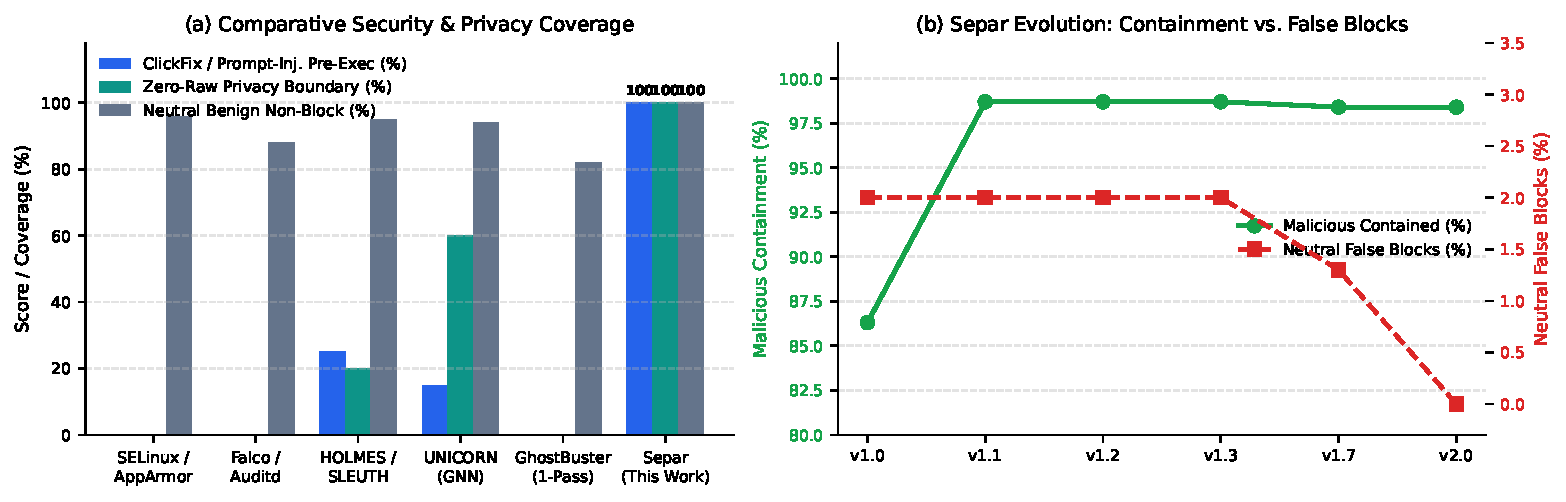
\includegraphics[width=0.85\textwidth]{figures/fig_comparative.pdf}
  \caption{(a)~Comparative security and privacy coverage across baselines (grounded in Tables~\ref{tab:rw_data}--\ref{tab:rw_method}); (b)~Separ's evolution from \texttt{v1.0} to \texttt{v2.0}, raising malicious containment to $98.4\%$ while driving neutral false blocks to $0.0\%$.}
  \label{fig:comparative}
\end{figure}

\paragraph{Comparative \& Evolution Analysis.} Figure~\ref{fig:comparative}(a) highlights why static MAC and additive rule engines fail on ClickFix/prompt-injection lures ($0\%$ pre-execution catch) and expose cleartext telemetry, whereas Separ achieves $100\%$ on both without blocking benign workflows. Figure~\ref{fig:comparative}(b) shows how eliminating uncontained holds (\texttt{v1.1}), enforcing posterior monotonicity (\texttt{v1.3}), and scoping trust marks to process lineage (\texttt{v2.0}) drove neutral false blocks down from $2.0\%$ to $0.0\%$.

\begin{figure}[!htbp]
  \centering
  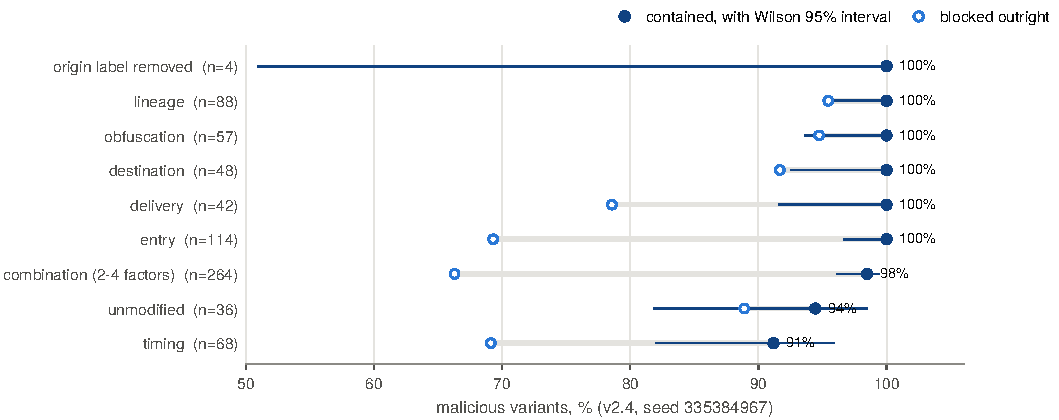
\includegraphics[width=0.68\textwidth]{figures/fig_dimensions.pdf}
  \caption{Mutation containment across all six perturbation dimensions and multi-factor combinations.}
  \label{fig:dimensions}
\end{figure}

\paragraph{Mutation Dimension Robustness.} As shown in Figure~\ref{fig:dimensions}, delivery, entry, obfuscation, destination, and lineage mutations are contained in $100\%$ of variants. Only extreme timing delays ($>30\,\text{min}$ gaps in slow ransomware \texttt{S19} and oversized response leaks \texttt{S27}) evade rate windows ($92.6\%$).

\begin{figure}[!htbp]
  \centering
  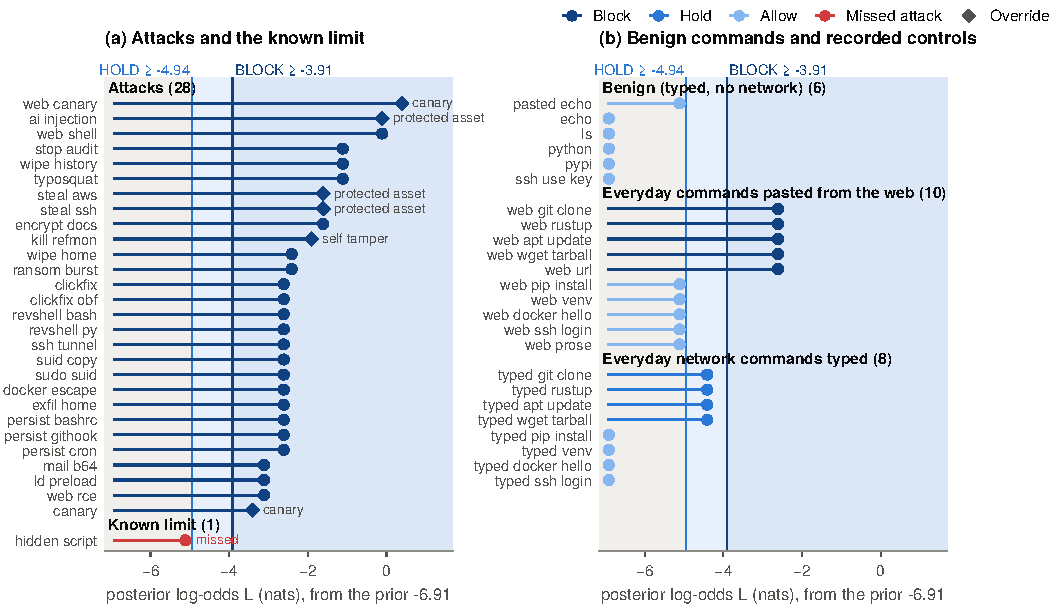
\includegraphics[width=0.72\textwidth]{figures/fig_lab_evidence.pdf}
  \caption{Bayesian evidence log-odds $L(S)$ across all 35 Attack Lab templates relative to $\tau_{\text{hold}}$ and $\tau_{\text{block}}$.}
  \label{fig:lab_evidence}
\end{figure}

\begin{figure}[!htbp]
  \centering
  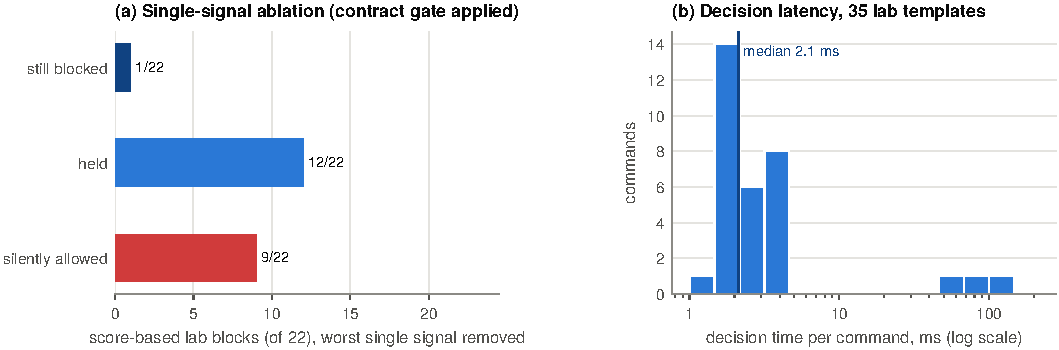
\includegraphics[width=0.72\textwidth]{figures/fig_lab_ablation_latency.pdf}
  \caption{(a)~Single-signal ablation on the 22 score-based Attack Lab blocks; (b)~per-command latency ($4.5\,\text{ms}$ median).}
  \label{fig:lab_ablation}
\end{figure}

\paragraph{Evidence Margins, Ablation, and Latency.} Figure~\ref{fig:lab_evidence} shows that score-based Attack Lab blocks average $+1.62\,\text{nats}$ above $\tau_{\text{block}}$, while harmless pasted controls sit safely at $-5.11\,\text{nats} < \tau_{\text{hold}}$. Figure~\ref{fig:lab_ablation}(a) confirms that removing any single Contract or Effect signal lets $9/22$ score-based blocks pass silently, proving that pasted attacks rely on predicted Effect. Figure~\ref{fig:lab_ablation}(b) shows $32/35$ decisions complete in under $10\,\text{ms}$ ($4.5\,\text{ms}$ median).

\begin{figure}[!htbp]
  \centering
  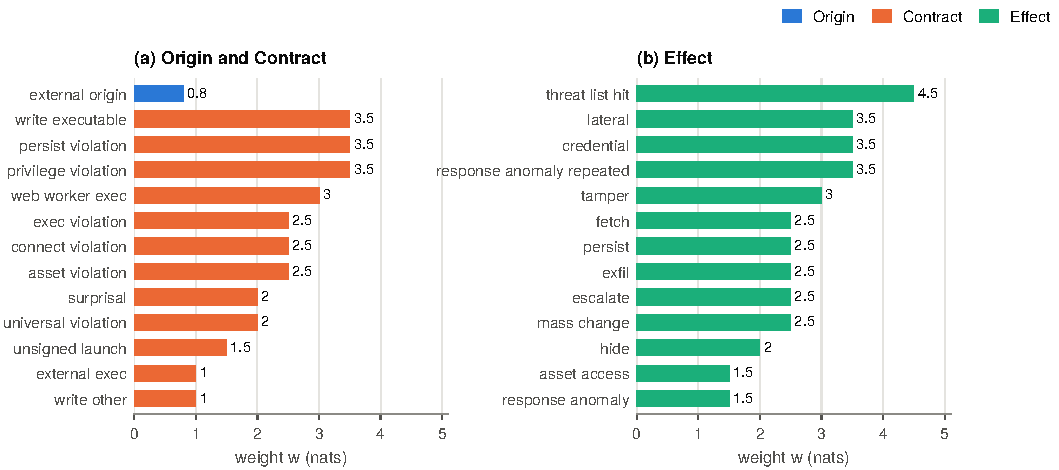
\includegraphics[width=0.58\textwidth]{figures/fig_weights.pdf}
  \caption{Frozen policy signal weights ($w_j$ in nats) grouped by Origin, Contract, and Effect.}
  \label{fig:weights}
\end{figure}

\end{document}
